\documentclass[11pt]{article}

\usepackage[T1]{fontenc}
\usepackage{lmodern}
\usepackage[margin=0.95in]{geometry}
\usepackage{amsmath,amssymb,amsthm}
\usepackage{array}
\usepackage{booktabs}
\usepackage{float}
\usepackage{graphicx}
\usepackage{microtype}
\usepackage{multirow}
\usepackage{natbib}
\usepackage{subcaption}
\usepackage{url}
\usepackage{xcolor}
\usepackage{hyperref}
\usepackage{tikz}

\usetikzlibrary{arrows.meta,positioning,shapes.geometric}
\hypersetup{
  colorlinks=true,
  citecolor=blue!55!black,
  linkcolor=blue!55!black,
  urlcolor=blue!55!black
}

\newcommand{\method}{AdaWP Code}
\newcommand{\mc}{Motion Code}
\newcommand{\R}{\mathbb{R}}
\newcommand{\softplus}{\operatorname{softplus}}
\newcommand{\softmax}{\operatorname{softmax}}
\newcommand{\best}[1]{\textbf{#1}}
\newcommand{\second}[1]{\textcolor{blue}{\underline{#1}}}
\newtheorem{proposition}{Proposition}

\title{Adaptive Warped Prototypes for Time Series Classification and Forecasting via Sparse Gaussian Processes}
\author{Sujato Dutta\\
Mahindra University
\and
Chandrajit Bajaj\\
The University of Texas at Austin}
\date{}

\begin{document}

\maketitle

\begin{abstract}
Gaussian-process time-series models provide useful structural representations, but their posterior means are not always reliable continuation rules beyond an observed prefix. We introduce \method{}, a template-guided adaptive warped prototype model for univariate classification and class-conditioned forecasting. Its central design principle is a division of labor: sparse Gaussian-process prototypes retain class-conditioned temporal structure and predictive variance, while a prefix-validated convex blend of stable dynamics heads supplies the forecast center. Ordered landmarks, bounded sample-conditioned residual codes, and monotonic temporal warps provide conservative alignment around each class prototype. Across 10 forecasting datasets, \method{} improves the published \mc{} RMSE on 9 tasks, with a 21.92\% mean relative reduction and a two-sided cross-dataset sign-test value of $p=0.0215$. The GP-only mean ablation increases relative RMSE by 650.92\%, directly supporting the proposed separation between probabilistic representation and extrapolation. Classification is retained as a secondary capability and evaluated against the original comparator suite and 11 locally evaluated neural baselines. We report predictive-interval calibration only as an appendix diagnostic because suffix shift remains unresolved.
\end{abstract}

\section{Introduction}

Forecasting beyond an observed prefix requires a model to answer two different questions. First, what temporal structure has the observed collection learned? Second, which continuation rule is stable outside the observed interval? A single flexible stochastic process need not answer both questions well. In particular, a Gaussian-process (GP) posterior can provide valuable class-conditioned structure and variance while its posterior mean becomes an unreliable extrapolator.

\mc{} \citep{bajaj2024motion} offers an interpretable starting point: class-associated sparse GPs and learned informative timestamps support both classification and forecasting. We retain that structural view but challenge the assumption that the GP posterior mean should also be the final forecast center. Our central idea is to assign representation and extrapolation to different mechanisms. Sparse GP prototypes model class-conditioned temporal structure. A nonnegative simplex blend of stable continuation heads supplies point forecasts, with blend weights selected only from rolling splits inside the observed prefix.

We call the resulting method \method{}, short for Template Guided Adaptive Warped Prototype Motion Code. The forecasting separation is the primary contribution. The model also introduces conservative alignment improvements: a bounded residual code, an ordered landmark decoder, and a monotonic temporal warp let each class prototype absorb within-class timing and amplitude variation without unconstrained sample-specific processes. Episodic generative-discriminative training and a validation-selected template head preserve classification capability.

The empirical pattern is sharp. On 10 class-conditioned forecasting datasets, \method{} improves the published \mc{} RMSE on 9 tasks, with a 21.92\% mean relative reduction. Replacing the dynamics blend with the GP mean increases relative RMSE by 650.92\%. Classification is secondary: on 12 datasets, the model maintains the original task performance while comparing favorably with 11 locally evaluated neural baselines. Predictive-interval calibration is reported as a diagnostic, not a solved contribution.

The contributions are:
\begin{itemize}
  \item a forecasting architecture that separates sparse-GP structural modeling from rolling-prefix selection of stable continuation dynamics;
  \item a conservative adaptive prototype parameterization with ordered landmarks, bounded residual motion codes, monotonic temporal alignment, and episodic generative-discriminative training;
  \item a reproducible evaluation with five-seed \method{} forecasting and classification tables, matched seed-42 DLinear and PatchTST forecasting references, 11 additional neural classification comparators, compact ablations, and explicit limitations.
\end{itemize}

\section{Related Work}

\paragraph{Time-series classification.}
The UCR archive \citep{dau2019ucr} supports reproducible comparison across diverse univariate classification problems. Classical approaches span elastic distances such as dynamic time warping \citep{keogh2005dtw}, interval forests \citep{deng2013tsf}, symbolic dictionaries such as BOSS \citep{schaefer2015boss}, canonical feature sets such as catch22 \citep{lubba2019catch22}, early classifiers such as TEASER \citep{schaefer2020teaser}, deep models such as LSTM-FCN \citep{karim2018lstmfcn}, random convolution methods such as ROCKET \citep{dempster2020rocket}, and heterogeneous ensembles such as HIVE-COTE 2.0 \citep{middlehurst2021hivecote}. The bake-off study of \citet{bagnall2017bakeoff} established a systematic evaluation tradition. We follow the comparator suite used by \mc{} so the new architecture can be measured against the model it extends.

\paragraph{Neural time-series backbones.}
Modern neural libraries expose a broad family of reusable temporal backbones. We evaluate retained classification runs for Informer \citep{zhou2021informer}, Autoformer \citep{wu2021autoformer}, FEDformer \citep{zhou2022fedformer}, ETSformer \citep{woo2022etsformer}, LightTS \citep{zhang2022lightts}, PatchTST \citep{nie2022patchtst}, Crossformer \citep{zhang2023crossformer}, DLinear \citep{zeng2023dlinear}, TimesNet \citep{wu2023timesnet}, iTransformer \citep{liu2024itransformer}, and Mamba \citep{gu2023mamba}. These models were originally motivated by different time-series or sequence-modeling regimes. We treat them as informative neural comparators under the common local classification assets, not as a claim that every architecture is a current state-of-the-art classifier.

Most of these architectures were designed for multivariate long-horizon forecasting. We include them as classification comparators where the retained local assets provide a meaningful common evaluation, but do not treat the full set as directly interchangeable forecasters for our short univariate class-conditioned protocol. To add matched neural forecasting references, we evaluate DLinear and PatchTST under the exact 80/20 protocol using sliding windows contained entirely within observed prefixes and without exposing final suffixes during training.

\paragraph{Sparse Gaussian processes.}
GPs provide calibrated probabilistic regression under a kernel prior \citep{rasmussen2006gaussian}. Sparse inducing-variable methods reduce the cost of inference while retaining an explicit posterior \citep{titsias2009variational}. Spectral-mixture kernels express stationary covariance as a learnable combination of interpretable frequency components \citep{wilson2013kernels}. \mc{} combines sparse GPs with learned informative timestamps. Our focus is complementary: we introduce conservative sample-conditioned alignment around class prototypes and separate GP variance from robust forecast centering.

\paragraph{Forecasting and predictive intervals.}
ARIMA, state-space models, and exponential smoothing remain important forecasting references \citep{box2015timeseries,harvey1990forecasting,delivera2011forecasting}. They also motivate our use of stable local continuation heads. Conformal regression methods construct predictive bands from held-out residuals with minimal modeling assumptions \citep{lei2018distribution}. For temporally ordered data, calibration design matters: suffix labels must not leak into model selection or scale fitting. Our exploratory appendix diagnostic therefore fits any variance rescaling only on rolling windows contained entirely within each observed prefix.

\section{Method}

\subsection{Problem Setting}

Let trajectory $i$ be an irregular univariate sequence
\begin{equation}
  X_i = \{(t_{ij}, y_{ij})\}_{j=1}^{n_i}, \qquad t_{ij}\in[0,1],
\end{equation}
with class label $c_i\in\{1,\ldots,C\}$. Values are robustly standardized using training-set median and interquartile range. For classification, we estimate $p(c_i\mid X_i)$. For forecasting, the collection class is known, following the class-conditioned \mc{} protocol, and the first 80\% of each trajectory is used to predict the final 20\%.

Figure~\ref{fig:architecture} summarizes the model. The central object is not one rigid process per class, but a class prototype with bounded sample-conditioned alignment.

\begin{figure}[H]
\centering
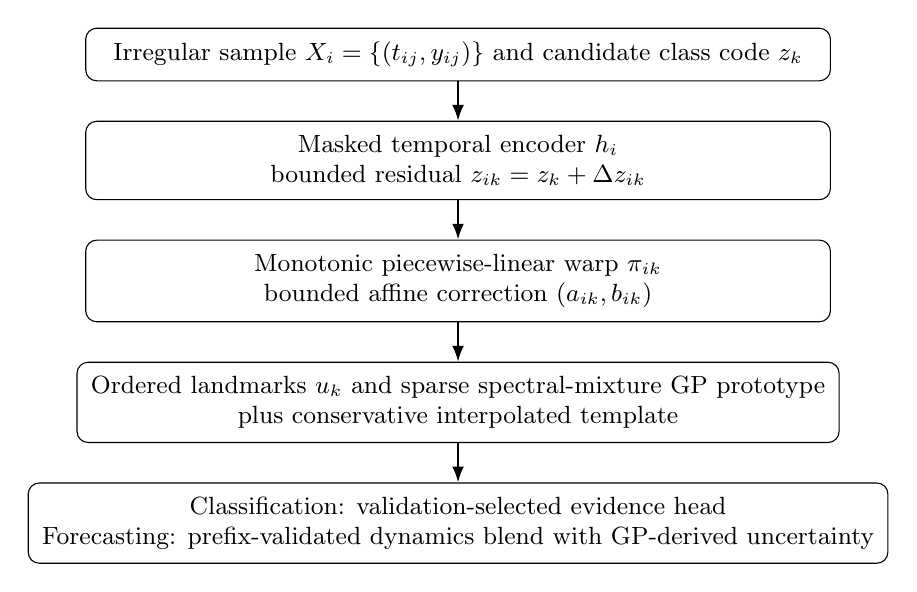
\begin{tikzpicture}[
  node distance=5mm,
  every node/.style={font=\small},
  box/.style={draw, rounded corners, align=center, inner sep=5pt, minimum width=0.78\linewidth},
  arrow/.style={-{Latex[length=2mm]}, thick}
]
  \node[box] (input) {Irregular sample $X_i=\{(t_{ij},y_{ij})\}$ and candidate class code $z_k$};
  \node[box, below=of input] (encoder) {Masked temporal encoder $h_i$\\bounded residual $z_{ik}=z_k+\Delta z_{ik}$};
  \node[box, below=of encoder] (align) {Monotonic piecewise-linear warp $\pi_{ik}$\\bounded affine correction $(a_{ik},b_{ik})$};
  \node[box, below=of align] (prototype) {Ordered landmarks $u_k$ and sparse spectral-mixture GP prototype\\plus conservative interpolated template};
  \node[box, below=of prototype] (output) {Classification: validation-selected evidence head\\Forecasting: prefix-validated dynamics blend with GP-derived uncertainty};
  \draw[arrow] (input) -- (encoder);
  \draw[arrow] (encoder) -- (align);
  \draw[arrow] (align) -- (prototype);
  \draw[arrow] (prototype) -- (output);
\end{tikzpicture}
\caption{\method{} architecture. Candidate-conditioned adaptation is bounded and the temporal warp is monotonic by construction.}
\label{fig:architecture}
\end{figure}

\subsection{Adaptive Motion Codes}

Each class $k$ owns a learned global motion code $z_k\in\R^d$. A masked temporal encoder summarizes the observed sample:
\begin{equation}
  h_i = \operatorname{Encoder}(X_i).
\end{equation}
The default encoder applies a pointwise multilayer perceptron, masked mean and max pooling, and compact temporal statistics. For every sample--class pair, an adapter predicts
\begin{align}
  \Delta z_{ik} &= \alpha\,\Delta_{\max}\tanh\!\left(f_\phi([h_i,z_k])\right),\\
  z_{ik} &= z_k + \Delta z_{ik},
\end{align}
where $\Delta_{\max}=0.20$ and $\alpha$ is warmed from zero to one over the first three training epochs. The residual is deliberately bounded. This permits within-class variation while preserving a stable neighborhood around the class prototype.

\subsection{Ordered Landmarks and Monotonic Warp}

Canonical informative times are decoded from positive gaps. With $m$ inducing landmarks and $m+1$ gaps,
\begin{align}
  g_k &= \softplus(g_{\mathrm{shared}} + f_{\mathrm{gap}}(z_k)) + \epsilon,\\
  u_{k,r} &= \frac{\sum_{\ell=1}^{r} g_{k,\ell}}{\sum_{\ell=1}^{m+1} g_{k,\ell}},
  \qquad r=1,\ldots,m.
\end{align}
Thus $0<u_{k,1}<\cdots<u_{k,m}<1$. We use $m=12$.

For a candidate class, the adapted code predicts positive warp-segment lengths through a softmax. Their cumulative sum defines increasing knots on $[0,1]$, and linear interpolation defines the sample-specific warp $\pi_{ik}$. Eight segments are used in all experiments. The model also predicts conservative amplitude and offset corrections:
\begin{equation}
  a_{ik}=\exp(0.20\tanh(s_{ik})), \qquad
  b_{ik}=0.30\tanh(o_{ik}).
\end{equation}
Observations are aligned as
\begin{equation}
  t'_{ij}=\pi_{ik}(t_{ij}), \qquad
  y'_{ij}=(y_{ij}-b_{ik})/a_{ik}.
\end{equation}
Regularizers penalize large residual codes, distorted warp gaps, extreme affine parameters, and poorly spaced canonical landmarks.

\subsection{Sparse GP Prototype}

Each class prototype uses a real spectral-mixture kernel:
\begin{equation}
  K_k(t,t') =
  \sum_{q=1}^{Q}
  \rho_{kq} A_q
  \exp\!\left(-2\pi^2 V_q(t-t')^2\right)
  \cos\!\left(2\pi F_q(t-t')\right),
  \label{eq:kernel}
\end{equation}
with $Q=4$ shared kernel atoms and nonnegative class-specific mixture weights $\rho_{kq}$. The ordered landmarks $u_k$ are inducing locations. Given aligned support trajectories, we infer a whitened sparse posterior with Cholesky solves and jitter $10^{-4}$. Computation uses double precision in the reported runs.

The prototype also includes a conservative template head. Support trajectories are RBF-interpolated onto a 96-point grid and averaged by class. The resulting template reconstruction error is useful when a flexible density score is unnecessarily sensitive to noise.

\subsection{Episodic Classification Objective}

Training uses class-balanced support--query episodes. A query is scored against class prototypes inferred from support trajectories; except for degenerate singleton classes, a query does not appear in its own support prototype. For query $i$, the model produces GP negative log density, GP mean-squared reconstruction error, template error, and encoder-centroid distance. Classification energy is converted to logits and optimized with cross entropy. The total objective is
\begin{equation}
  \mathcal{L} =
  \mathcal{L}_{\mathrm{CE}}
  + \lambda_{\mathrm{gen}}\mathcal{L}_{\mathrm{GP\text{-}NLL}}^{\mathrm{true}}
  + \mathcal{R},
 \qquad \lambda_{\mathrm{gen}}=0.15,
 \label{eq:objective}
\end{equation}
where $\mathcal{R}$ collects structural regularizers. This objective combines discrimination with a proper generative pressure: the true class process must continue to explain the observed trajectory.

After training, the evidence head is selected using validation trajectories only. Candidate heads are evaluated in the fixed order template, GP-NLL, and GP-MSE; accuracy ties retain the earlier, simpler head. Test labels never influence this choice.

\subsection{Class-Conditioned Forecasting}

Direct GP-mean extrapolation is unstable for some long suffixes. We retain GP posterior variance but estimate the forecast center using stable continuations. Let $\widehat{y}_{ih}^{(r)}$ be the horizon-$h$ prediction from head $r$. Candidate heads include persistence, moving means, seasonal naive rules, damped drift, damped Holt trend, local autoregressions, Fourier continuation, and pooled global or class autoregressions. The point forecast is
\begin{equation}
  \widehat{y}_{ih} = \sum_{r=1}^{R} w_r\widehat{y}_{ih}^{(r)},
  \qquad w_r\geq 0,\quad \sum_{r=1}^{R}w_r=1.
  \label{eq:blend}
\end{equation}
Weights are fitted by ridge-regularized least squares on rolling origins at prefix fractions $\{0.45,0.55,0.65,0.75\}$. Each internal target spans 25\% of the available prefix. The final suffix remains untouched until evaluation.

The sparse GP posterior continues to emit class-conditioned predictive variance as an auxiliary output. Appendix~\ref{app:calibration} evaluates a prefix-only conformal rescaling diagnostic. We do not treat that rescaling as a contribution because it does not reliably resolve final-suffix distribution shift.

\section{Experimental Setup}

\paragraph{Datasets.}
Classification uses 12 datasets: two Parkinson sensor settings, PronunciationAudio, and nine UCR datasets. Forecasting uses 10 datasets: PronunciationAudio and the nine UCR datasets. Table~\ref{tab:data} in Appendix~\ref{app:execution} gives train/test sizes, class counts, and sequence lengths. UCR data follow the archive definition \citep{dau2019ucr}. PronunciationAudio is constructed from the released clean audio assets.

\paragraph{Protocols.}
Classification uses the released train/test partitions. Within the training set, 20\% is reserved for validation head and checkpoint selection. The main classification table reports seeds 42--46, 30 epochs, one episodic step per epoch, at most 16 support and 8 query samples per class, and no scratch refit. Forecasting uses the released class-conditioned clean 80/20 protocol: the first 80\% of every trajectory is observed and the final 20\% is forecast. The class label is available to the forecaster. Forecast point predictions are deterministic given the dataset; five-seed runs verify that training randomness does not change the retained forecast result.

\paragraph{Baselines and provenance.}
For classification, we include the comparator suite reported with \mc{}: DTW, TSF, RISE, BOSS, BOSS-E, catch22, Shapelet, TEASER, SVC, LSTM-FCN, ROCKET, HIVE-COTE 2.0, and \mc{}. We additionally extract 11 complete neural comparator columns from retained TSLibrary classification result files on the same dataset assets. Each neural comparator column is a single retained run; \method{} reports five seeds. For forecasting, we include exponential smoothing, ARIMA, state-space, persistence, TBATS, \mc{}, and matched local DLinear and PatchTST references. The classical and \mc{} values from the original \mc{} manuscript and released benchmark artifacts are reference values, not newly rerun matched-environment measurements. DLinear and PatchTST are locally evaluated with seed 42 using one TSLibrary model per known class and sliding windows fully contained in observed prefixes. Our main \method{} forecasting values retain five seeds.

\paragraph{Metrics and statistics.}
Classification uses test accuracy. Forecasting uses root mean squared error (RMSE), where lower is better. We report the unweighted mean effect over datasets, a dataset-bootstrap 95\% interval for the mean forecast improvement, and a two-sided sign test across forecasting datasets. Dataset-level resampling is the unit of bootstrap analysis.

\section{Results}

\subsection{Forecasting}

Forecasting is the primary result. Table~\ref{tab:forecast-main} reports RMSE against the original forecasting suite and two matched neural references. \method{} improves the published \mc{} value on 9 of 10 datasets. Relative RMSE reduction averages 21.92\%, with median 14.46\% and dataset-bootstrap 95\% interval $[10.00,35.37]$. The two-sided sign-test value for 9 wins in 10 tasks is $p=0.0215$. The largest relative reductions are on InsectEPGRegularTrain (60.21\%), SonyAIBORobotSurface2 (54.88\%), and Lightning7 (38.18\%). PronunciationAudio is the one regression, from 0.085 to 0.087 RMSE.

The neural references make the comparison more informative without changing the conclusion. PatchTST is strongest on HouseTwenty and second on SonyAIBORobotSurface2; DLinear is second on PowerCons. \method{} is strongest on 5 of 10 tasks, while TBATS is strongest on three, persistence on one, and PatchTST on one. This distribution supports evaluating stable dynamics and neural forecasters together rather than assuming a single family dominates every short suffix.

\begin{table}[H]
\centering
\caption{Class-conditioned forecasting RMSE; lower is better. DLinear and PatchTST are matched local seed-42 TSLibrary runs trained only on prefix-contained windows. The classical and \mc{} columns are reported reference values; \method{} reports the retained five-seed result. Bold marks the best result and blue underlining marks the second best.}
\label{tab:forecast-main}
\scriptsize
\resizebox{\textwidth}{!}{%
\begin{tabular}{lrrrrrrrrr}
\toprule
Dataset & Exponential smoothing & ARIMA & State space & Persistence & TBATS & DLinear & PatchTST & \mc{} & \method{} \\
\midrule
PronunciationAudio        & 0.087 & 0.087 & 0.086 & 0.100 & \best{0.059} & 0.099 & 0.148 & \second{0.085} & 0.087 \\
ECGFiveDays               & 0.310 & 0.260 & 0.240 & \second{0.190} & \best{0.170} & 0.536 & 1.133 & 0.270 & 0.253 \\
FreezerSmallTrain         & 0.730 & 0.790 & 0.860 & \second{0.570} & \best{0.560} & 0.999 & 0.883 & 0.740 & 0.690 \\
HouseTwenty               & 872.790 & 904.470 & 663.320 & \second{497.300} & 726.520 & 582.115 & \best{490.215} & 648.270 & 527.170 \\
InsectEPGRegularTrain     & 0.021 & 0.033 & 0.084 & \best{0.019} & 0.025 & 0.031 & 0.025 & 0.048 & \second{0.019} \\
ItalyPowerDemand          & 1.400 & 1.340 & 1.030 & 1.240 & 0.960 & 0.952 & 1.105 & \second{0.670} & \best{0.537} \\
Lightning7                & 1.350 & 1.100 & 1.370 & 1.350 & \second{1.060} & 1.375 & 2.014 & 1.080 & \best{0.668} \\
MoteStrain                & 1.180 & 1.390 & 1.320 & 1.010 & 1.120 & 0.945 & 0.927 & \second{0.820} & \best{0.763} \\
PowerCons                 & 1.510 & 2.140 & 2.260 & 1.770 & 1.130 & \second{1.086} & 1.278 & 1.150 & \best{1.032} \\
SonyAIBORobotSurface2     & 2.170 & 3.580 & 2.780 & 1.390 & 1.800 & 1.241 & \second{1.231} & 2.260 & \best{1.020} \\
\bottomrule
\end{tabular}}
\end{table}

\subsection{Ablations}

Table~\ref{tab:forecast-ablations} isolates the forecasting design. The strongest single ablation is also the clearest statement of the paper's novelty: replacing the prefix-validated dynamics blend with the GP posterior mean increases average relative RMSE by 650.92\%. The GP prototype remains useful for structural modeling and auxiliary variance, but it should not be forced to serve as the extrapolation center.

The smaller ablations refine that conclusion. Restricting the model to local-only dynamics increases mean relative RMSE by 9.40\%, showing that conservatively pooled collection dynamics help. Persistence is strong on individual tasks and beats the final blend on 4 of 10 datasets, but increases average relative RMSE by 7.00\%. The simplex blend therefore earns its complexity by selecting among stable continuations without abandoning simple rules when they are useful.

\begin{table}[H]
\centering
\caption{Seed-42 forecasting ablations. Effects are mean relative RMSE changes versus the full prefix-validated blend; positive is worse. ``GP-only posterior mean'' removes the stable continuation heads and centers the forecast directly on sparse-GP extrapolation. Bold marks the best result and blue underlining marks the second best.}
\label{tab:forecast-ablations}
\small
\begin{tabular}{lrr}
\toprule
Forecasting variant & Rel.\ RMSE change & Better/tied/worse \\
\midrule
Full prefix-validated blend   & \best{0.000\%}    & 0/10/0 \\
Local-only dynamics           & +9.405\%   & 2/5/3 \\
Persistence                   & \second{+7.001\%}   & 4/0/6 \\
GP-only posterior mean        & +650.925\% & 0/0/10 \\
\bottomrule
\end{tabular}
\end{table}

\subsection{Classification Retention}

Classification is a retained capability rather than the paper's primary claim. Tables~\ref{tab:neural-classification-a} and~\ref{tab:neural-classification-b} compare \method{} with 11 complete TSLibrary neural comparator columns. Results vary by dataset, so we do not present classification as a broad advance. Table~\ref{tab:classification-full} provides the complete reported comparator suite, including \mc{}. Appendix~\ref{app:classification-ablation} reports secondary classifier ablations.

\begin{table}[H]
\centering
\caption{Classification accuracy (\%), neural comparators I. Informer is the ProbSparse Transformer; Autoformer uses decomposition and auto-correlation; FEDformer is the frequency-enhanced decomposed Transformer; ETSformer is the exponential-smoothing Transformer; LightTS is the light sampling-oriented MLP. Comparator columns are retained TSLibrary runs on the common assets. \method{} reports mean $\pm$ standard deviation over seeds 42--46. Bold marks the best result and blue underlining marks the second best across both neural-comparator tables.}
\label{tab:neural-classification-a}
\scriptsize
\resizebox{\textwidth}{!}{%
\begin{tabular}{lrrrrrr}
\toprule
Dataset & Informer & Autoformer & FEDformer & ETSformer & LightTS & \method{} \\
\midrule
PDSetting1                & 67.70 & 56.21 & 66.46 & 59.63 & 66.15 & \best{70.50 $\pm$ 0.00} \\
PDSetting2                & \best{53.85} & 35.20 & 47.55 & 39.63 & 47.55 & \second{53.10 $\pm$ 0.80} \\
PronunciationAudio        & 68.75 & 68.75 & 75.00 & \second{87.50} & 68.75 & \best{88.75 $\pm$ 8.15} \\
ECGFiveDays               & 53.66 & 57.72 & 58.19 & 59.93 & 55.87 & \best{67.36 $\pm$ 2.44} \\
FreezerSmallTrain         & 58.84 & 51.79 & 50.98 & 61.09 & 61.33 & \best{70.32 $\pm$ 0.71} \\
HouseTwenty               & 62.18 & 58.82 & 57.98 & \best{69.75} & 63.87 & \second{66.39 $\pm$ 2.30} \\
InsectEPGRegularTrain     & \best{100.00} & 47.39 & 46.18 & 77.91 & \second{91.57} & \best{100.00 $\pm$ 0.00} \\
ItalyPowerDemand          & 74.73 & 73.66 & \best{76.97} & 74.44 & 71.62 & 72.38 $\pm$ 0.73 \\
Lightning7                & 27.40 & 26.03 & 28.77 & 26.03 & 30.14 & \second{37.26 $\pm$ 4.27} \\
MoteStrain                & 61.98 & 51.76 & 52.24 & 64.30 & 57.43 & \best{72.68 $\pm$ 0.00} \\
PowerCons                 & 90.56 & 55.56 & 62.22 & 84.44 & 93.33 & 92.67 $\pm$ 1.59 \\
SonyAIBORobotSurface2     & 73.56 & 75.55 & 76.18 & 75.24 & 74.40 & \second{76.39 $\pm$ 0.00} \\
\bottomrule
\end{tabular}}
\end{table}

\begin{table}[H]
\centering
\caption{Classification accuracy (\%), neural comparators II. PatchTST is the patch-based Transformer; Crossformer uses cross-dimension dependency; DLinear is the decomposition linear model; TimesNet models temporal 2D variation; iTransformer is the inverted Transformer; Mamba is the selective state-space model. Comparator columns are retained TSLibrary runs on the common assets. \method{} reports mean $\pm$ standard deviation over seeds 42--46. Bold marks the best result and blue underlining marks the second best across both neural-comparator tables.}
\label{tab:neural-classification-b}
\scriptsize
\resizebox{\textwidth}{!}{%
\begin{tabular}{lrrrrrrr}
\toprule
Dataset & PatchTST & Crossformer & DLinear & TimesNet & iTransformer & Mamba & \method{} \\
\midrule
PDSetting1                & 58.07 & \second{70.19} & 66.77 & 68.63 & 69.88 & 68.94 & \best{70.50 $\pm$ 0.00} \\
PDSetting2                & 36.83 & \best{53.85} & 51.28 & 51.75 & 50.35 & 47.55 & \second{53.10 $\pm$ 0.80} \\
PronunciationAudio        & 75.00 & 81.25 & \second{87.50} & 75.00 & 81.25 & 75.00 & \best{88.75 $\pm$ 8.15} \\
ECGFiveDays               & 56.45 & 59.00 & \second{60.28} & 55.17 & 56.91 & 54.59 & \best{67.36 $\pm$ 2.44} \\
FreezerSmallTrain         & 56.21 & 60.63 & \second{65.23} & 56.21 & 63.68 & 57.33 & \best{70.32 $\pm$ 0.71} \\
HouseTwenty               & 60.50 & 54.62 & 59.66 & 63.03 & 63.03 & 60.50 & \second{66.39 $\pm$ 2.30} \\
InsectEPGRegularTrain     & 49.80 & \best{100.00} & 83.53 & \best{100.00} & 85.54 & \best{100.00} & \best{100.00 $\pm$ 0.00} \\
ItalyPowerDemand          & 71.14 & 76.68 & \second{76.87} & 73.66 & 75.02 & 75.90 & 72.38 $\pm$ 0.73 \\
Lightning7                & 27.40 & 28.77 & \best{39.73} & 28.77 & 27.40 & 26.03 & \second{37.26 $\pm$ 4.27} \\
MoteStrain                & 58.55 & 59.19 & \second{66.85} & 60.30 & 63.02 & 60.86 & \best{72.68 $\pm$ 0.00} \\
PowerCons                 & 86.67 & \second{94.44} & 92.78 & 93.89 & 92.78 & \best{95.00} & 92.67 $\pm$ 1.59 \\
SonyAIBORobotSurface2     & 74.82 & \best{76.60} & 73.56 & 71.67 & 75.87 & 76.18 & \second{76.39 $\pm$ 0.00} \\
\bottomrule
\end{tabular}}
\end{table}

\begin{table}[H]
\centering
\caption{Complete reported classification comparison and five-seed \method{} accuracy (\%). DTW is dynamic time warping; TSF is time-series forest; RISE is random interval spectral ensemble; BOSS is bag-of-SFA-symbols; BOSS-E is its ensemble; SVC is support-vector classification; LSTM-FCN is the long short-term memory fully convolutional network; ROCKET uses random convolutional kernels; HC2 is HIVE-COTE 2.0. A dash indicates an unavailable comparator entry. Bold marks the best result and blue underlining marks the second best.}
\label{tab:classification-full}
\tiny
\resizebox{\textwidth}{!}{%
\begin{tabular}{lrrrrrrrrrrrrrr}
\toprule
Dataset & DTW & TSF & RISE & BOSS & BOSS-E & catch22 & Shapelet & TEASER & SVC & LSTM-FCN & ROCKET & HC2 & \mc{} & \method{} \\
\midrule
PDSetting1            & 63.35 & 63.98 & \second{70.81} & 61.80 & 65.53 & 68.94 & 52.80 & 59.94 & 63.96 & 43.48 & 61.49 & 59.63 & \best{71.12} & 70.50 $\pm$ 0.00 \\
PDSetting2            & 43.12 & 51.98 & \second{53.61} & 45.92 & 36.83 & 51.52 & 44.99 & 37.53 & 48.02 & 24.01 & 51.52 & 50.82 & \best{54.31} & 53.10 $\pm$ 0.80 \\
PronunciationAudio    & 50.00 & \second{87.50} & 62.50 & 68.75 & 62.50 & 50.00 & 68.75 & -- & 62.50 & 56.25 & 75.00 & 75.00 & \second{87.50} & \best{88.75 $\pm$ 8.15} \\
ECGFiveDays           & 54.47 & 58.07 & 59.35 & 50.06 & 58.42 & 52.85 & 52.61 & -- & 49.71 & 53.54 & 56.79 & 55.75 & \second{66.55} & \best{67.36 $\pm$ 2.44} \\
FreezerSmallTrain     & 52.42 & 54.28 & 53.79 & 50.00 & 50.95 & 53.58 & 50.00 & 50.11 & 50.00 & 50.00 & 52.67 & 58.18 & \second{70.25} & \best{70.32 $\pm$ 0.71} \\
HouseTwenty           & 57.98 & 57.14 & 42.02 & 52.10 & 57.98 & 45.38 & 57.14 & 53.78 & 45.38 & 57.98 & 58.82 & 59.66 & \best{70.59} & \second{66.39 $\pm$ 2.30} \\
InsectEPGRegularTrain & \best{100.00} & \best{100.00} & 83.13 & \second{99.20} & 91.97 & 95.98 & 44.58 & \best{100.00} & 85.94 & \best{100.00} & 46.18 & \best{100.00} & \best{100.00} & \best{100.00 $\pm$ 0.00} \\
ItalyPowerDemand      & 57.05 & 68.71 & 65.79 & 52.77 & 53.26 & 55.88 & 62.49 & 63.17 & 49.85 & 61.61 & 70.36 & \best{72.98} & \second{72.50} & 72.38 $\pm$ 0.73 \\
Lightning7            & 21.92 & 28.77 & 26.03 & 12.33 & 28.77 & 24.66 & 20.55 & 21.92 & 26.03 & 17.81 & 27.40 & \second{32.88} & 31.51 & \best{37.26 $\pm$ 4.27} \\
MoteStrain            & 56.47 & 61.10 & 61.50 & 53.83 & 53.51 & 57.19 & 47.76 & -- & 50.64 & 56.55 & 68.85 & 56.95 & \second{72.68} & \best{72.68 $\pm$ 0.00} \\
PowerCons             & 78.33 & 92.22 & 85.56 & 65.56 & 77.22 & 80.00 & 74.44 & 51.11 & 77.78 & 68.33 & 87.22 & 90.00 & \best{92.78} & \second{92.67 $\pm$ 1.59} \\
SonyAIBORobotSurface2 & 63.27 & 67.68 & 69.78 & 48.06 & 61.91 & 64.43 & 69.36 & 68.84 & 61.70 & 63.27 & 74.71 & \best{78.49} & 75.97 & \second{76.39 $\pm$ 0.00} \\
\bottomrule
\end{tabular}}
\end{table}

\section{Discussion and Limitations}

\method{} is built around one forecasting insight: probabilistic temporal structure and stable extrapolation are related but distinct responsibilities. The GP-only ablation demonstrates that distinction directly. Sparse prototypes remain useful as compact class-conditioned representations, while rolling-prefix validation selects a robust continuation center from deliberately simple dynamics. The adaptive residual and warp are supporting engineering choices: they preserve conservative alignment and classification capability, but their separate classification ablations do not justify presenting them as the main empirical breakthrough.

Several limitations remain. Forecasting is class-conditioned: the collection label is known at prediction time. The reported 10 datasets form a focused evaluation rather than an exhaustive long-horizon forecasting benchmark. Comparator values inherited from the \mc{} manuscript are reference values rather than fresh matched-hardware reruns. Classification is retained, not materially advanced over \mc{}. Finally, GP-derived variance remains an auxiliary output rather than a calibrated uncertainty contribution. Appendix~\ref{app:calibration} documents that prefix-only rescaling can still fail under suffix shift.

\section{Conclusion}

We presented \method{}, a forecasting-oriented adaptive warped prototype model. Its central principle is to retain sparse-GP prototypes for temporal structure while selecting the point-forecast center from stable continuation dynamics validated inside the observed prefix. This separation improves published \mc{} RMSE on 9 of 10 forecasting datasets, and the GP-only ablation shows why the distinction matters. Ordered landmarks, bounded residual codes, monotonic alignment, and validation-only classification-head selection preserve the original classification capability. Reliable uncertainty adjustment under suffix shift remains future work.

\clearpage
\bibliographystyle{plainnat}
\bibliography{references}

\appendix

\section{Construction Properties}
\label{app:proofs}

\begin{proposition}[Strictly ordered canonical landmarks]
If each decoded gap $g_{k,\ell}$ is strictly positive, then the inducing landmarks satisfy
$0<u_{k,1}<\cdots<u_{k,m}<1$.
\end{proposition}
\begin{proof}
Each numerator $\sum_{\ell=1}^{r}g_{k,\ell}$ is positive and strictly increases with $r$. It is strictly smaller than the denominator $\sum_{\ell=1}^{m+1}g_{k,\ell}$ because one positive terminal gap remains. Dividing by the positive denominator preserves order and places all landmarks strictly inside $(0,1)$.
\end{proof}

\begin{proposition}[Monotonic temporal alignment]
The piecewise-linear map $\pi_{ik}$ is strictly increasing on $[0,1]$.
\end{proposition}
\begin{proof}
Warp-segment logits are mapped through softmax, so every segment length is positive and the lengths sum to one. Their cumulative sums therefore define strictly increasing knots with endpoints 0 and 1. Linear interpolation between adjacent increasing knots has positive slope on every segment, hence $\pi_{ik}$ is strictly increasing.
\end{proof}

\begin{proposition}[Positive semidefinite prototype kernel]
The kernel in Eq.~\eqref{eq:kernel} is positive semidefinite when $A_q\geq0$, $V_q\geq0$, and $\rho_{kq}\geq0$.
\end{proposition}
\begin{proof}
For each atom $q$, the factor
$\exp(-2\pi^2 V_q\tau^2)\cos(2\pi F_q\tau)$
is the stationary covariance associated with a symmetric pair of Gaussian spectral components centered at $\pm F_q$, with $\tau=t-t'$. It is therefore positive semidefinite by Bochner's theorem. A nonnegative weighted sum of positive semidefinite kernels is positive semidefinite.
\end{proof}

\begin{proposition}[No held-out-suffix leakage]
Forecast blend weights and conformal variance scales do not use values from the final evaluation suffix.
\end{proposition}
\begin{proof}
For each trajectory, the outer protocol first fixes the observed 80\% prefix. Rolling-origin design matrices, residuals, and GP-derived variances are then constructed using splits wholly contained inside that prefix. Equation~\eqref{eq:blend} and the conformal quantile are fitted from these inner splits only. The final 20\% suffix is read only after fitting for metric computation.
\end{proof}

\paragraph{Coverage scope.}
The preceding proposition is a leakage statement, not an unconditional coverage theorem for future suffixes. Standard split-conformal marginal coverage relies on exchangeability of calibration and test nonconformity scores \citep{lei2018distribution}. Temporal suffix shift can violate this condition, as reflected by the diagnostic failures in Table~\ref{tab:calibration-full}.

\section{Execution and Reproducibility Details}
\label{app:execution}

\paragraph{Core configuration.}
All reported \method{} runs use 12 inducing landmarks, latent code dimension 8, four spectral atoms, encoder hidden width 64, encoder output width 32, adapter hidden width 64, eight warp segments, maximum residual magnitude 0.20, GP jitter $10^{-4}$, minimum noise 0.03, a 96-point template grid, and double-precision PyTorch tensors. The classification generative weight is 0.15. Structural regularization weights are $10^{-2}$ for residual norm, $10^{-2}$ for warp distortion, $10^{-3}$ for affine correction, $2\cdot10^{-3}$ for gap regularity, and $10^{-4}$ for class-code norm.

\paragraph{Classification protocol.}
The retained paper runs use seeds 42, 43, 44, 45, and 46; 30 epochs; one episode per epoch; 20\% validation fraction; 25\% query fraction; at most 16 support and 8 query trajectories per class; evaluation batch size 64; and no scratch refit. The adapter is warmed over three epochs. Checkpoint and evidence-head selection use the validation partition only.

\paragraph{Forecasting protocol.}
Each observed prefix contains the first 80\% of a training trajectory. Point-forecast blend weights are fitted only from inner rolling origins $\{0.45,0.55,0.65,0.75\}$ with internal horizon fraction 0.25 and blend ridge 0.02. Pooled autoregressions are enabled conservatively for short prefixes. The appendix diagnostic fits a prefix-only conformal variance scale with nominal interval target 0.95.

\paragraph{Neural classification comparators.}
The 11 neural comparator columns in Tables~\ref{tab:neural-classification-a} and~\ref{tab:neural-classification-b} are extracted from complete retained TSLibrary \texttt{result\_classification.txt} files using \texttt{extract\_tslibrary\_classification\_results.py}. Each column contains one result per retained classification dataset. The generated evidence file is \texttt{out/awp\_paper\_evidence/tslibrary\_classification\_baselines.csv}.

\paragraph{Neural forecasting comparators.}
DLinear and PatchTST use the unchanged TSLibrary model implementations through \texttt{benchmark\_tslibrary\_neural\_forecasting.py}. For each known collection class, the adapter trains one model on sliding input--target windows contained entirely within the observed 80\% prefixes. The evaluation suffix is not used for training, model selection, or normalization. Both comparator columns report seed 42 with 10 training epochs, a maximum receptive field of 96, and at most 256 windows per trajectory. PatchTST uses model width 128, feed-forward width 256, three encoder layers, and eight attention heads, matching the retained TSLibrary classification capacity.

\paragraph{Software record.}
The retained audit was generated on Windows with Python 3.11.9, NumPy 2.4.6, and PyTorch 2.12.0+cpu. CUDA was unavailable for these runs. The reproducibility package records SHA-256 hashes for code, classification assets, forecasting assets, and result completeness: 60 classification JSON files, 50 forecasting JSON files, 84 classification-ablation rows, and 40 forecasting-ablation rows.

\begin{table}[H]
\centering
\caption{Classification dataset sizes and lengths. Variable-length Parkinson settings report minimum and maximum lengths.}
\label{tab:data}
\small
\resizebox{\textwidth}{!}{%
\begin{tabular}{lrrrrr}
\toprule
Dataset & Train & Test & Classes & Min.\ length & Max.\ length \\
\midrule
PDSetting1                & 20  & 322  & 2 & 257 & 1665 \\
PDSetting2                & 24  & 429  & 3 & 208 & 1665 \\
PronunciationAudio        & 16  & 16   & 2 & 100 & 100 \\
ECGFiveDays               & 23  & 861  & 2 & 136 & 136 \\
FreezerSmallTrain         & 28  & 2850 & 2 & 301 & 301 \\
HouseTwenty               & 40  & 119  & 2 & 2000 & 2000 \\
InsectEPGRegularTrain     & 62  & 249  & 3 & 601 & 601 \\
ItalyPowerDemand          & 67  & 1029 & 2 & 24 & 24 \\
Lightning7                & 70  & 73   & 7 & 319 & 319 \\
MoteStrain                & 20  & 1252 & 2 & 84 & 84 \\
PowerCons                 & 180 & 180  & 2 & 144 & 144 \\
SonyAIBORobotSurface2     & 27  & 953  & 2 & 65 & 65 \\
\bottomrule
\end{tabular}}
\end{table}

\begin{table}[H]
\centering
\caption{Forecasting dataset sizes. Forecasting uses the class-conditioned clean 80/20 protocol on the training collections.}
\label{tab:forecast-data}
\small
\begin{tabular}{lrrrr}
\toprule
Dataset & Trajectories & Classes & Observed length & Future length \\
\midrule
PronunciationAudio        & 16  & 2 & 80   & 20 \\
ECGFiveDays               & 23  & 2 & 108  & 28 \\
FreezerSmallTrain         & 28  & 2 & 240  & 61 \\
HouseTwenty               & 40  & 2 & 1600 & 400 \\
InsectEPGRegularTrain     & 62  & 3 & 480  & 121 \\
ItalyPowerDemand          & 67  & 2 & 19   & 5 \\
Lightning7                & 70  & 7 & 255  & 64 \\
MoteStrain                & 20  & 2 & 67   & 17 \\
PowerCons                 & 180 & 2 & 115  & 29 \\
SonyAIBORobotSurface2     & 27  & 2 & 52   & 13 \\
\bottomrule
\end{tabular}
\end{table}

\section{Secondary Classification Ablations}
\label{app:classification-ablation}

Table~\ref{tab:classification-ablation} reports seed-42 classifier ablations. Removing the generative term in Eq.~\eqref{eq:objective} reduces average accuracy by 3.73 percentage points. The bounded adaptive residual and temporal warp have much smaller average effects, $-0.02$ and $-0.22$ points when removed. These components are conservative alignment mechanisms rather than the primary source of the forecasting improvement.

\begin{table}[H]
\centering
\caption{Seed-42 classification ablations. Effects are mean accuracy changes in percentage points versus the full classifier. Bold marks the best result and blue underlining marks the second best.}
\label{tab:classification-ablation}
\small
\begin{tabular}{lrr}
\toprule
Classification variant & Mean accuracy & $\Delta$ vs.\ full \\
\midrule
Full \method{}                & \best{73.497} & 0.000 \\
No adaptive residual          & \second{73.481} & -0.017 \\
No temporal warp              & 73.280 & -0.217 \\
No generative loss            & 69.764 & -3.733 \\
Fixed template inference      & 73.391 & -0.106 \\
Fixed NLL inference           & 71.296 & -2.201 \\
Fixed MSE inference           & 71.919 & -1.578 \\
\bottomrule
\end{tabular}
\end{table}

\section{Predictive-Interval Diagnostic}
\label{app:calibration}

The sparse GP posterior emits predictive variance as an auxiliary output. We evaluate a post-hoc prefix-only split-conformal rescaling diagnostic without claiming it as a solved calibration method. On rolling-prefix residuals, define
\begin{equation}
  r_\ell=\frac{|e_\ell|}{\sqrt{v_\ell}},
\end{equation}
where $v_\ell$ is GP-derived variance. The finite-sample conformal quantile of $r_\ell$ rescales final interval width without reading the held-out suffix. Table~\ref{tab:calibration-full} shows why the result remains diagnostic: scaling improves several datasets, but FreezerSmallTrain deteriorates from 68.97\% to 45.15\% coverage and other suffixes remain under-covered. Prefix-only fitting prevents leakage; it does not eliminate temporal distribution shift.

\begin{table}[H]
\centering
\caption{Exploratory nominal 95\% predictive-interval coverage. Interval width is measured in each dataset's original value scale.}
\label{tab:calibration-full}
\small
\resizebox{\textwidth}{!}{%
\begin{tabular}{lrrrr}
\toprule
Dataset & Before conformal & Prefix conformal & Abs.\ target error & Mean interval width \\
\midrule
PronunciationAudio        & 98.12\% & 99.67\% & 4.67 pp  & 0.759 \\
ECGFiveDays               & 100.00\% & 100.00\% & 5.00 pp & 6.846 \\
FreezerSmallTrain         & 68.97\% & 45.15\% & 49.85 pp & 0.334 \\
HouseTwenty               & 93.11\% & 98.30\% & 3.30 pp  & 4077.724 \\
InsectEPGRegularTrain     & 100.00\% & 100.00\% & 5.00 pp & 1.588 \\
ItalyPowerDemand          & 81.86\% & 86.66\% & 8.34 pp  & 2.414 \\
Lightning7                & 91.02\% & 94.60\% & 0.40 pp  & 3.693 \\
MoteStrain                & 94.35\% & 94.41\% & 0.59 pp  & 2.856 \\
PowerCons                 & 68.05\% & 80.19\% & 14.81 pp & 3.113 \\
SonyAIBORobotSurface2     & 68.35\% & 77.88\% & 17.12 pp & 3.509 \\
\bottomrule
\end{tabular}}
\end{table}

\section{Representative Landmark Visualizations}
\label{app:visualizations}

Figure~\ref{fig:baseline-landmarks} provides representative landmark and extrapolation visualizations from the released \mc{} implementation. They motivate the landmark-based design inherited by \method{}; they are not used as quantitative evidence for the new architecture.

\begin{figure}[H]
\centering
\begin{subfigure}{0.48\textwidth}
  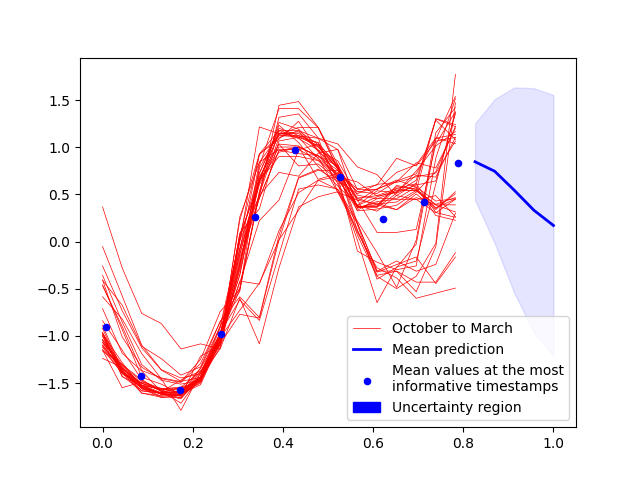
\includegraphics[width=\linewidth]{figures/ItalyPowerDemand0.png}
  \caption{ItalyPowerDemand example.}
\end{subfigure}
\hfill
\begin{subfigure}{0.48\textwidth}
  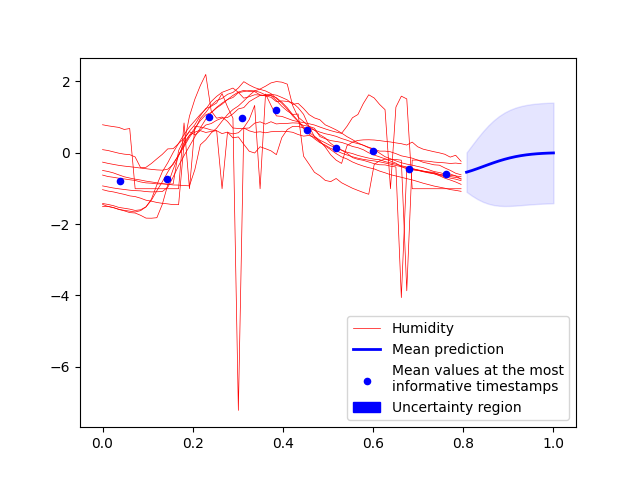
\includegraphics[width=\linewidth]{figures/MoteStrain0.png}
  \caption{MoteStrain example.}
\end{subfigure}

\medskip
\begin{subfigure}{0.48\textwidth}
  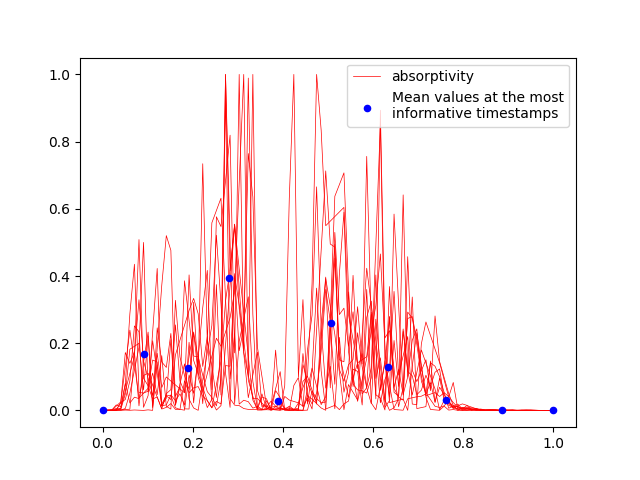
\includegraphics[width=\linewidth]{figures/test_audio0.png}
  \caption{PronunciationAudio example.}
\end{subfigure}
\hfill
\begin{subfigure}{0.48\textwidth}
  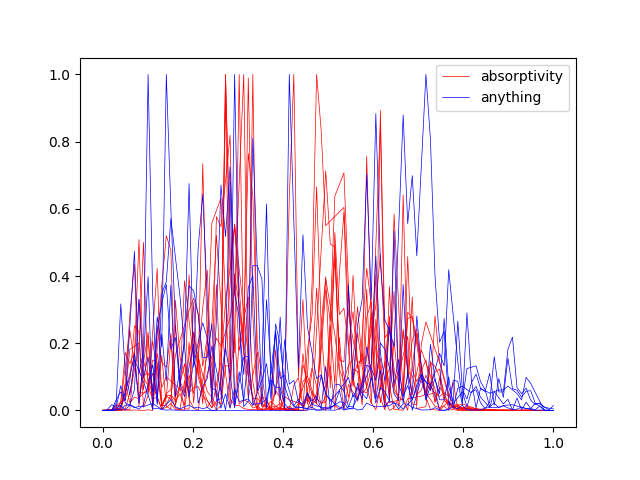
\includegraphics[width=\linewidth]{figures/plot_train_test_audio.png}
  \caption{PronunciationAudio collection view.}
\end{subfigure}
\caption{Representative released-\mc{} landmark visualizations. Blue landmark markers identify informative timestamps; forecast panels show predictive continuation and uncertainty where applicable.}
\label{fig:baseline-landmarks}
\end{figure}

\section{Artifact Map}
\label{app:artifact}

The implementation is organized around a small set of entry points. The core architecture is in \texttt{awp\_motion\_code.py}. Dataset definitions and reported reference values are in \texttt{awp\_datasets.py}. Classification training and aggregation are in \texttt{benchmark\_awp\_motion\_code.py} and \texttt{aggregate\_awp\_results.py}. Forecast loading, stable dynamics heads, simplex fitting, and conformal diagnostics are in \texttt{awp\_forecasting\_utils.py}; forecasting evaluation and aggregation are in \texttt{benchmark\_awp\_forecasting.py} and \texttt{aggregate\_awp\_forecasts.py}. The matched TSLibrary neural forecast adapter is \texttt{benchmark\_tslibrary\_neural\_forecasting.py}. Ablation entry points are \texttt{run\_awp\_classification\_ablation.py} and \texttt{evaluate\_cached\_awp\_forecasting.py}. The command \texttt{extract\_tslibrary\_classification\_results.py} regenerates the neural classification comparison CSV from retained TSLibrary files. The command \texttt{generate\_awp\_paper\_evidence.py} regenerates statistical summaries, coverage tables, environment metadata, and the reproducibility audit from cached outputs.

\end{document}
